\chapter{Przypadki użycia}

\section{Diagram przypadków użycia}

\begin{figure}[h!] 
\centering
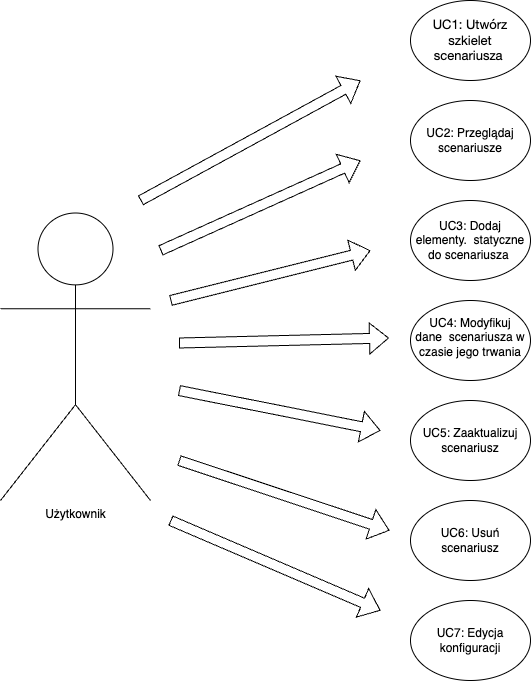
\includegraphics[width=0.8\textwidth]{resources/local/use-case-diagram.png}
\caption{Diagram przypadków użycia} 
\label{fig:use_case_diagram}
\end{figure}

\section{Tabela przypadków użycia}

\begin{longtable}{|p{1cm}|p{5cm}|p{9cm}|}
\caption{Tabela przypadków użycia} \label{tab:use_case_table} \\ % Umieść podpis tutaj
\hline
\textbf{ID} & \textbf{Przypadek użycia} & \textbf{Opis} \\
\hline
\endfirsthead
\caption[]{Tabela przypadków użycia -- ciąg dalszy} \\ % Powtarzany podpis dla następnych stron
\hline
\textbf{ID} & \textbf{Przypadek użycia} & \textbf{Opis} \\
\hline
\endhead
\hline
\endfoot
\hline
\endlastfoot
UC1 & Utwórz szkielet scenariusza & Użytkownik tworzy scenariusz podając jego czas wraz z pozostałymi właściwościami go opisującymi. System dodaje nowy scenariusz wraz z domyślnymi danymi tworzonymi dla nowego scenariusza. \\
\hline
UC2 & Przeglądaj scenariusze & Użytkownik przegląda listę dostępnych scenariuszy, z opcją filtrowania, która umożliwia wybranie konkretnego scenariusza oraz jego edycję lub usunięcie. \\
\hline
UC3.1 & Utwórz szablon obiektu & Użytkownik tworzy szablon obiektu dostępny we wszystkich scenariuszach. \\
\hline
UC3.3 & Utwórz obiekt & Użytkownik tworzy konkretny obiekt przypisany do scenariusza. \\
\hline
UC3.4 & Utwórz szablon atrybutu & Użytkownik tworzy szablon atrybutu przyporządkowany do danego szablonu obiektu. \\
\hline
UC3.5 & Utwórz atrybut & Użytkownik tworzy atrybut dla konkretnego obiektu. \\
\hline
UC3.2 & Utwórz typ obiektu & Użytkownik tworzy typ obiektu dostępny we wszystkich scenariuszach. \\
\hline
UC3.6 & Utwórz typ asocjacji & Użytkownik tworzy typ asocjacji dostępny we wszystkich scenariuszach. \\
\hline
UC3.7 & Utwórz asocjację & Użytkownik tworzy asocjację pomiędzy dwoma obiektami z danego scenariusza. \\
\hline
UC4.1 & Utwórz wątek & Użytkownik tworzy nowy wątek poprzez rozdzielenie wątku istniejącego lub dodanie nowego osobnego wątku. \\
\hline
UC4.2 & Utwórz zdarzenie & Użytkownik tworzy zdarzenie wraz ze zdefiniowaniem zmian w asocjacjach lub atrybutach obiektów. \\
\hline
UC5.1 & Edycja danych podanych przy tworzeniu scenariusza & Użytkownik modyfikuje właściwości scenariusza podane podczas jego tworzenia. \\
\hline
UC5.2 & Edycja elementów statycznych oraz zdarzeń & Użytkownik modyfikuje istniejące elementy statyczne (np. obiekty, atrybuty) wraz z właściwościami zdarzeń i wątków. \\
\hline
UC.6 & Usuń scenariusz & Użytkownik usuwa scenariusz po jego wybraniu z listy. System pyta o potwierdzenie i usuwa scenariusz wraz z danymi prywatnymi dla scenariusza na stałe. \\
\hline
UC.7 & Edycja konfiguracji & Użytkownik edytuje konfigurację. System wykorzystuje zdefiniowane właściwości przy tworzeniu nowego scenariusza. \\
\hline
\end{longtable}


